\documentclass{article}
% \documentclass[twocolumn]{article}

\title{Batch Correlation in Mixnets: Computing Mapping Probabilities}

\author{Aiswarya Walter, Student ID: 427199}

\date{}

%%packages
\usepackage[margin=1.5cm,nohead]{geometry}
\usepackage{graphicx}
\usepackage{dblfloatfix} 
\usepackage{amsmath}
\usepackage[colorlinks=true, allcolors=blue]{hyperref}
\usepackage{algorithm}
\usepackage{algpseudocode}
\usepackage{float} 
\algnewcommand\algorithmicforeach{\textbf{for each}}
\algdef{S}[FOR]{ForEach}[1]{\algorithmicforeach\ #1\ \algorithmicdo}
\usepackage{caption}  
\usepackage{afterpage}
\usepackage{placeins}  % For \FloatBarrier
\usepackage{needspace}

\makeatletter
\renewcommand{\ALG@name}{}  % Remove "Algorithm" text
\renewcommand{\thealgorithm}{Phase \arabic{algorithm}}  % Change numbering to "Phase X"
\makeatother

% Float parameters
\renewcommand{\topfraction}{0.9}
\renewcommand{\bottomfraction}{0.8}
\setcounter{topnumber}{2}
\setcounter{bottomnumber}{2}
\setcounter{totalnumber}{4}
\renewcommand{\dbltopfraction}{0.9}
\setcounter{dbltopnumber}{2}

\begin{document}

\maketitle

\section{Problem Definition}
\label{sec:problem}

Mix networks (mixnets) are anonymous communication systems that 
provide privacy protection by preventing 
adversaries from tracing communication patterns and 
linking senders to recipients. Unlike low-latency 
systems such as Tor, mixnets introduce deliberate 
delays and message mixing strategies to ensure 
 unlinkability even against powerful 
adversaries capable of global network monitoring. 
They operate by routing messages through a series 
of intermediary nodes known as mixes, which 
shuffle and delay packets to disrupt any 
correlation between input and output messages, 
making it difficult for observers to correlate 
incoming and outgoing traffic patterns.

One critical challenge in mixnet design is handling node failures, which 
can compromise message delivery and system reliability. One of the strategies 
to address this challenge is message splitting, where a single  
message is divided into multiple sub-messages that are sent as a batch. 
The original message can be reconstructed when a sufficient number of 
sub-messages in the batch are successfully received at the destination, 
typically using erasure coding or redundancy schemes. This approach 
provides fault tolerance by allowing message recovery even when some 
sub-messages are lost, while maintaining the mixing properties of 
the network.

The challenge arises when a global adversary observes 
the mixnet system. Such an adversary can monitor all incoming and outgoing 
traffic at the mix nodes, recording message arrival and departure timestamps, 
batch compositions, and routing patterns. This batch-level 
correlation problem is particularly challenging because 
temporal patterns, batch sizes, and network timing constraints can leak 
information about the mapping between input and output batches. Even 
though individual messages within batches may be cryptographically 
protected, the observable metadata (timing, message counts) 
can be exploited to reduce the anonymity provided by the mixnet.

\textbf{Problem Statement:} Given a mixnet system operating with
message batches under observation by a global adversary, the aim is to develop 
an algorithm that computes the probability 
that each observed outgoing batch corresponds to each possible incoming 
batch, considering timing constraints and batch coherence requirements.

\subsection{Assumptions}
\label{sec:assumptions}

The proposed batch matching algorithm in Section~\ref{sec:solution}
operates under several assumptions:

\begin{itemize}
\item The model assumes no message loss during transmission, 
reliable mix nodes without failures, crashes, or Byzantine 
behavior. In practice, networks experience failures, 
congestion, and malicious behavior that would 
impact batch reconstruction and correlation analysis.

\item The model assumes fixed batch sizes and predictable 
processing patterns. Real mixnets may employ variable batch sizes, 
padding, dummy messages, and complex 
batching strategies that could alter correlation 
patterns and anonymity properties.

\item The model does not include countermeasures such as 
traffic padding, cover traffic, dummy messages, or other 
defensive techniques that real mixnets might deploy to 
enhance anonymity against traffic analysis attacks.

\item The adversary is assumed to have perfect global observation 
with complete visibility into all incoming and outgoing traffic 
and precise timestamps. This may not reflect realistic monitoring 
constraints or partial network visibility.

\item The evaluation focuses on a single Poisson mix node 
rather than more complex multi-hop mixnet topologies that 
could provide additional anonymity guarantees.
\end{itemize}

\subsection{Anonymity Metrics}
\label{sec:anonymity_metrics}

The following anonymity metrics are used to quantify the 
privacy provided by mixnet systems:

\begin{itemize}
\item \textbf{Batch Mapping Probabilities:} The probability 
that each outgoing batch originated 
from each possible incoming 
batch, representing the uncertainty an adversary faces when 
attempting to correlate batches.

\item \textbf{Anonymity Set:} The collection of incoming batches 
that could plausibly have contributed to a given outgoing batch. 
Larger anonymity sets indicate stronger privacy protection.

\item \textbf{Anonymity Set Size:} The number of possible incoming 
batches for each outgoing batch, which is the cardinality of the 
anonymity set of the given outgoing batch.

\end{itemize}

\section{Proposed Solution: The Mixnet Batch Matching Algorithm}
\label{sec:solution}


% \vspace{1em} 
\begin{table*}[!htbp]
\centering\footnotesize 
\begin{tabular}{l p{5.5cm} p{5.5cm}}
\hline
\textbf{Variables and Functions} & \textbf{Description} & \textbf{Data Type} \\
\hline
$M_{ij}$      & $j$-th message in the incoming batch $i$ & Message object\\
$O_{pq}$      & $q$-th message in the outgoing batch $p$ & Message object\\
$t_{M_{ij}}$  & Arrival time of message $M_{ij}$ & Timestamp  \\
$t_{O_{pq}}$  & Sending time of message $O_{pq}$ & Timestamp  \\
$IncomingBatches$ & Mapping of incoming batch ids to its messages & Dictionary of dictionaries \\
$OutgoingBatches$ & Mapping of outgoing batch ids to its messages & Dictionary of dictionaries \\
$OutBatchMappingCount$ & For each outgoing batch, it maps the candidate incoming batches to the number of valid permutations to that batch & Dictionary of dictionaries \\
$OutMsgMappingSet$ & Set of valid input messages for each outgoing message, $O_{pq}$ & Dictionary of sets of messages \\
$Valids$      & List of valid message permutations for all outgoing batches & List of dictionaries of lists  \\
$BatchProb$ & Probability mapping for all output batches & Dictionary of dictionaries \\
$AnonymitySet$ & Set of incoming batches that contribute to the anonymity of each outgoing batch & Dictionary of sets of messages \\
$AnonymitySetSize$ & Number of incoming batches that could have contributed to each outgoing batch & Dictionary of integers \\
$batchid(msg)$ & Returns the batch id of the message  & Function (returns integer) \\
$msgid(msg)$   & Returns the message id  & Function (returns integer) \\
$appendMsg(subpermutation, msg)$  & Operation to append a message to an existing sup-permutation of a batch  & Function (returns list) \\
\hline
\end{tabular}
\caption{Algorithm variables and functions.} % (add a caption; helps placement)
\label{tab:variables}
\end{table*}

The Mixnet Batch Matching algorithm addresses the batch 
correlation problem by systematically enumerating 
all valid message-to-batch mappings and computing 
probability distributions for each outgoing batch. 
The algorithm operates incrementally, processing 
each outgoing message as it enters a batch and 
updating the global set of valid permutations 
(see $Valids$ in Table~\ref{tab:variables}).

One of the algorithm's main data structures is a batch mapping 
\textbf{permutation} (elements of $Valids$), 
which represents a complete assignment of incoming messages to outgoing 
batch positions. Specifically, each permutation is a mapping from 
outgoing batch IDs to lists of incoming messages, where 
each list represents the possible source incoming messages that could 
have contributed to that outgoing batch.

For example, consider a scenario with three outgoing batches (A, B, C) 
and incoming messages from batches 1, 2, and 3. A valid permutation might be:
\begin{align}
\text{Permutation} = \{&\text{A}: [M_{11}, M_{12}], \\
                      &\text{B}: [M_{21}], \\
                      &\text{C}: [M_{31}, M_{32}, M_{33}]\}
\end{align}

This permutation hypothesizes that outgoing batch A originated 
from two messages in incoming batch 1, outgoing batch B came 
from one message in incoming batch 2, and outgoing batch C 
derived from three messages in incoming batch 3.

Each individual mapping within a permutation 
(e.g., \text{A}: [$M_{11}$, $M_{12}$]) 
is called a \textbf{sub-permutation}, representing the 
specific assignment of incoming messages to a single 
outgoing batch position. Each outgoing batch has its own 
sub-permutation defining which incoming messages could 
have contributed to it.


The algorithm maintains two constraints for valid permutations:

\begin{itemize}
\item All messages mapped to the same outgoing batch must 
originate from the same incoming batch. 

\item Only incoming messages that arrived before an outgoing 
message was sent can be candidates for mapping to that 
outgoing batch, ensuring realistic timing relationships.
\end{itemize}

The algorithm explores all permutations that satisfy 
these constraints, counting how many valid mappings exist for 
each outgoing-to-incoming batch pair. The final probability 
that outgoing batch $p$ originated from incoming batch $i$ is computed as:

$$P(\text{outgoing batch } p \leftarrow \text{incoming batch } i) = \frac{\text{number of valid permutations mapping } p \text{ to } i}{\text{total number of valid permutations}}$$


Table~\ref{tab:variables} provides a comprehensive 
overview of the key variables, data structures, 
and functions used throughout the algorithm. 
The algorithm maintains several core data 
structures: \texttt{Valids} stores the current 
set of valid permutations, \texttt{OutBatchMappingCount} 
tracks the number of valid mappings for each 
outgoing-incoming batch pair, \texttt{BatchProb} 
contains the final probability distributions, 
and \texttt{OutMsgMappingSet} holds the eligible 
incoming messages for each outgoing batch. The algorithm 
also maintains anonymity-related structures: 
\texttt{AnonymitySet} stores the set of incoming batches 
that could have contributed to each outgoing batch, 
while \texttt{AnonymitySetSize} records the cardinality 
of these anonymity sets for privacy quantification. 
The helper functions \texttt{batchid()} and \texttt{msgid()} 
extract batch and message identifiers respectively, 
while \texttt{appendMsg()} handles the creation of 
extended sub-permutations during the permutation 
expansion phase.

The following subsections describe each phase of the algorithm in detail, providing both pseudocode and comprehensive explanations of the underlying logic.



\subsection{Initialization and Candidate Selection}

~\ref{alg:phase1} sets up the fundamental data 
structures and identifies eligible messages for 
batch mapping. In lines 1-4, the algorithm 
initializes empty containers for the core data 
structures: \texttt{Valids} for storing valid 
permutations, \texttt{BatchProb} for probability 
distributions, and \texttt{AnonymitySet} 
and \texttt{AnonymitySetSize} for anonymity metrics. 
Line 5 records the arrival of outgoing 
message $O_{pq}$ in batch $p$ at timestamp $t_{O_{pq}}$, and line 6 
initializes the \texttt{OutMsgMappingSet[$O_{pq}$]}
as an empty set to store eligible incoming messages 
for the current outgoing message.

Lines 7-13 implement the candidate selection 
logic by iterating through all incoming batches 
and applying size-based filtering. For each 
incoming batch $i$, the algorithm compares 
its size ($lenIn$) with the current outgoing 
batch size ($lenOut$) in line 10. Only 
incoming batches that satisfy the 
constraint $lenIn \geq lenOut$ are 
considered as candidates (line 11). This creates the 
initial structure \texttt{OutBatchMappingCount[p][i]} 
with a count of zero for each eligible incoming batch.

The temporal filtering occurs in lines 14-20, 
where the algorithm examines each message in the 
candidate incoming batches. Lines 14-15 establish 
nested loops that iterate through each eligible 
incoming batch $i$ in \texttt{OutBatchMappingCount[p]} 
and each message $M_{ij}$ with timestamp $t_{M_{ij}}$ 
in that batch. For every such message, the algorithm 
applies the causality 
constraint $t_{M_{ij}} < t_{O_{pq}}$ (line 16). 
Only messages that arrived before the current 
outgoing message was sent are added 
to \texttt{OutMsgMappingSet[$O_{pq}$]} (line 17), 
ensuring temporal consistency in the batch mapping.


\begin{algorithm}
\caption{Initialization and Candidate Selection}
\label{alg:phase1}
\begin{algorithmic}[1]
\State $Valids \gets [] $
\State $BatchProb \gets \{ \} $
\State $ AnonymitySet \gets \{ \} $
\State $ AnonymitySetSize \gets \{ \} $
\State Outgoing message $O_{pq}$ enters the outgoing batch, $p$ at time $t_{O_{pq}}$
\State $OutMsgMappingSet [O_{pq}] \gets \{ \} $
\ForEach{$ i \text{ in } IncomingBatches $}
    \State $ lenIn \gets len(IncomingBatches[i]) $
    \State $ lenOut \gets len(OutgoingBatches[p]) $
    \If{$ lenIn \geq  lenOut $}
        \State $OutBatchMappingCount[p][i] \gets 0 $
    \EndIf
\EndFor
\ForEach{$ i \text{ in } OutBatchMappingCount[p] $}
    \ForEach{$ M_{ij}, t_{M_{ij}} \text{ in } IncomingBatches[i] $}
        \If{$ t_{M_{ij}} < t_{O_{pq}} $}
            \State $ OutMsgMappingSet[O_{pq}].add(M_{ij}) $
        \EndIf
    \EndFor
\EndFor
\end{algorithmic}
\end{algorithm}

\subsection{Initial Permutation Construction}

% old text:
% ~\ref{alg:phase2} handles the base case when no valid 
% permutations have been established yet. 
% For each eligible incoming message identified 
% in Phase 1, the algorithm creates a new permutation 
% where that message is mapped to the current outgoing 
% batch position, establishing the initial set of 
% valid mappings that will be expanded in subsequent phases.

~\ref{alg:phase2} handles the base case 
when no valid permutations have been established 
yet. Line 1 checks if the \texttt{Valids} list 
is empty, indicating this is the first outgoing 
message being processed. In this scenario, 
lines 2-4 iterate through each eligible incoming 
message $M_{ij}$ from the $OutMsgMappingSet[O_{pq}]$
collection established in ~\ref{alg:phase1}.

For each eligible message, line 3 creates a new 
permutation represented as a dictionary where 
the key $p$ (the current outgoing batch ID) 
maps to a list containing the single 
message $M_{ij}$. This creates the foundational 
permutation structure $\{p: [M_{ij}]\}$ that will 
be expanded in subsequent phases. Each such 
permutation is appended to the \texttt{Valids} 
list, establishing the initial set of valid 
mappings that serve as the basis for all future 
extensions.


\begin{algorithm}[H]
\caption{Initial Permutation Construction}
\label{alg:phase2}
\begin{algorithmic}[1]
\If{$Valids = [ ] $}
    \ForEach{$M_{ij} \in OutMsgMappingSet[O_{pq}]$}
        \State $Valids \gets Valids.append(\{ p: [M_{ij}] \} )$
    \EndFor
\EndIf
\end{algorithmic}
\end{algorithm}

\subsection{Permutation Extension and Validation}

~\ref{alg:phase3} implements the core 
expansion logic when valid permutations 
already exist. Line 1 checks that 
\texttt{Valids} is not empty, confirming 
that initial permutations have been established. 
Line 2 initializes \texttt{tempValids} as a 
temporary container for the new set of 
extended permutations.

Lines 3-5 begin the message processing 
loop, where each eligible incoming 
message $M_{ij}$ is extracted along 
with its batch ID ($i$) and message ID ($j$) 
using the helper functions \texttt{batchid()} 
and \texttt{msgid()}. Lines 7-9 initialize 
the permutation extension variables: \texttt{newX} 
as a copy of the current permutation $x$, \texttt{count} 
as a validation counter, and \texttt{msgList} 
as the existing sub-permutation for outgoing 
batch $p$.

The algorithm handles two distinct cases 
based on whether a sub-permutation already 
exists for batch $p$. In Case 1 (lines 10-29), 
when \texttt{msgList} exists, lines 12-20 
implement the coherence validation logic. 
The inner loop examines each 
existing message in the sub-permutation, 
extracting its batch ID ($b$) and message ID ($m$) 
in lines 13-14. The coherence 
check occurs in line 15: if all existing 
messages come from the same incoming 
batch ($b = i$) and the new message is 
distinct ($m \neq j$), the count is 
incremented; otherwise, the validation 
fails and the loop breaks.

If the coherence check passes (line 21), 
indicating all messages in the sub-permutation 
plus the new message belong to the same 
incoming batch, lines 22-26 extend the 
sub-permutation by appending $M_{ij}$ 
using \texttt{appendMsg()}, updating the 
permutation structure, adding it 
to \texttt{tempValids}, and incrementing 
the mapping count for batch pair $(p,i)$.

Case 2 (lines 30-45) handles the creation 
of new sub-permutations when no mapping 
exists for batch $p$. Lines 32-36 implement 
the uniqueness constraint by checking that 
incoming batch $i$ has not been used 
elsewhere in the current permutation. 
If batch $i$ is unique across the entire 
permutation (line 37), lines 38-40 create 
a new sub-permutation containing only $M_{ij}$, 
add the extended permutation to \texttt{tempValids}, 
and update the mapping count.

Lines 48-49 finalize the phase by replacing 
the old \texttt{Valids} with the newly 
constructed \texttt{tempValids} and resetting 
the temporary container for the next iteration.



\begin{algorithm}
\caption{Permutation Extension and Validation}
\label{alg:phase3}
\begin{algorithmic}[1]
\If{$Valids \neq [] $}
    \State $tempValids \gets []$
    \ForEach{$M_{ij} \in OutMsgMappingSet[O_{pq}]$}
        \State $ i \gets batchid(M_{ij}) $
        \State $ j \gets msgid(M_{ij}) $
        \ForEach{$x \text{ in} Valids$}
            \State $ newX \gets x $
            \State $count \gets 0$
            \State $ msgList \gets newX.get(p) $
            \If {$ msgList $ exists}
                \State \Comment{Case 1: Extend existing sub-permutation}
                \For{$v \gets 0$ to $len(msgList)$}
                    \State $ b \gets batchid(msgList[v]) $
                    \State $ m \gets msgid(msgList[v]) $
                    \If{$ b = i$ \textbf{and} $ m \neq j $}
                        \State $count \gets count + 1$
                    \Else
                        \State \textbf{break}
                    \EndIf
                \EndFor
                \If{$count = len(msgList)$}
                    \State $ newMsgList \gets appendMsg( msgList,M_{ij})$
                    \State $newX[p] \gets newMsgList $
                    \State $tempValids \gets tempValids.append(newX)$
                    \State $ OutBatchMappingCount[p][i] \gets OutBatchMappingCount[p][i] + 1$
                    \State $count \gets 0$
                \Else
                    \State $count \gets 0$
                \EndIf
            \Else
                \State \Comment{Case 2: Create new sub-permutation}
                \ForEach{$ batchMsgs \text{ in } x $}
                    \If{$\text{batchid}(batchMsgs[0]) \neq i$}
                        \State $count \gets count + 1$
                    \EndIf
                \EndFor
                \If{$count = len(x) $}
                    \State $newX [p] \gets  [M_{ij}] $
                    \State $ tempValids \gets tempValids.append(newX) $
                    \State $ OutBatchMappingCount[p][i] \gets OutBatchMappingCount[p][i] + 1 $
                    \State $count \gets 0$
                \Else
                    \State $count \gets 0$
                \EndIf
            \EndIf
        \EndFor
    \EndFor
    \State $ Valids \gets tempValids $
    \State $ tempValids \gets [] $
\EndIf
\end{algorithmic}
\end{algorithm}

\subsection{Global Batch Mapping Update}

~\ref{alg:phase4} ensures consistency 
across all outgoing batch mappings after the 
current batch has been processed. Lines 1-2 
establish nested loops that iterate through 
every valid permutation $x$ in \texttt{Valids} 
and every outgoing batch ID (\texttt{outid}) 
within each permutation.

Line 3 implements a filtering condition to 
skip the current batch $p$, focusing only on 
previously processed outgoing batches that 
need count updates. For qualifying batches, 
line 4 extracts the incoming batch ID (\texttt{inId}) 
from the first message in the sub-permutation, leveraging 
the batch coherence property that ensures all 
messages in a sub-permutation originate from 
the same incoming batch.

Line 5 performs the count increment 
operation by updating \texttt{OutBatchMappingCount[outid][inId]}, 
ensuring that the mapping counts for all 
outgoing batches remain synchronized with 
the current set of valid permutations. 
This maintains the integrity of probability 
calculations across the entire system.


\begin{algorithm}[H]
\caption{Global Batch Mapping Update}
\label{alg:phase4}
\begin{algorithmic}[1]
\ForEach{$x \text{ in } Valids$}
    \ForEach{$ outid \text{ in } x $}
        \If{$ outid \neq p $}
            \State $ inId \gets \text{batchid}(x[outid][0])$
            \State $ OutBatchMappingCount[outid][inId] \gets OutBatchMappingCount[outid][inId] + 1$
        \EndIf
    \EndFor
\EndFor
\end{algorithmic}
\end{algorithm}

\subsection{Probability Computation and Finalization}

~\ref{alg:phase5} computes the final 
probability distributions and anonymity 
metrics. Lines 2-5 iterate through all 
outgoing batches in \texttt{OutBatchMappingCount}, 
initializing empty probability dictionaries for 
new batches and creating a \texttt{nonZero} 
container for valid mappings.

Lines 6-11 implement the probability calculation 
logic for each incoming-outgoing batch pair. 
Line 7 computes the probability as the fraction of 
valid permutations that map 
the incoming batch to the outgoing batch. 
Lines 8-10 filter out zero probabilities, 
storing only meaningful mappings in \texttt{nonZero}.

Lines 12-20 handle the finalization of results 
based on whether valid mappings exist. 
If \texttt{nonZero} contains valid mappings (line 12), 
lines 13-15 populate the final data 
structures: \texttt{BatchProb} receives the 
probability distribution, \texttt{AnonymitySet} 
stores the set of contributing incoming batches, 
and \texttt{AnonymitySetSize} records the 
cardinality of the \texttt{AnonymitySet}. 
If no valid mappings exist (lines 16-19), 
any existing entries for the outgoing batch 
are removed from \texttt{BatchProb}.

Lines 22-25 reset the global data structures 
to prepare for processing the next outgoing 
message, clearing \texttt{OutBatchMappingCount}, 
\texttt{BatchProb}, \texttt{AnonymitySet}, 
and \texttt{AnonymitySetSize} to ensure a 
clean state for subsequent iterations.

\begin{algorithm}
\caption{Probability Computation and Finalization}
\label{alg:phase5}
\begin{algorithmic}[1]
\ForEach{$ outBatch \text{ in } OutBatchMappingCount $}
    \If{$ outBatch  \text{ not in } BatchProb $}
        \State $ BatchProb[outBatch] \gets \{ \} $
    \EndIf
    \State $ nonZero \gets \{ \} $
    \ForEach{$(inBatch, count) \text{ in } OutBatchMappingCount[outBatch] $}
        \State $ prob \gets \frac{count}{len(Valids)}$
        \If{$ prob  > 0 $}
            \State $ nonZero[inBatch] \gets prob $
        \EndIf
    \EndFor
    \If{$ nonZero $}
        \State $ BatchProb[outBatch] \gets nonZero $
        \State $ AnonymitySet[outBatch] \gets \{ nonZero.keys() \} $
        \State $ AnonymitySetSize[outBatch] \gets len(AnonymitySet[outBatch]) $
    \Else
        \If{$ outBatch \text{ in } BatchProb $}
            \State $ del BatchProb[outBatch] $
        \EndIf
    \EndIf
\EndFor
\State $OutBatchMappingCount \gets \{ \} $
\State $ BatchProb \gets \{ \} $
\State $ AnonymitySet \gets \{ \} $
\State $ AnonymitySetSize \gets \{ \} $
\end{algorithmic}
\end{algorithm}

\section{Evaluation}
\label{sec:evaluation}

To assess the proposed Mixnet Batch Matching 
algorithm, we implemented it within a mixnet simulation framework 
called Mixim. The evaluation focuses on understanding how various 
system parameters affect anonymity metrics under the global 
adversary model.

\subsection{Evaluation Metrics}
\label{sec:metrics}

The evaluation involves three anonymity metrics 
to assess the privacy guarantees provided by the 
mixnet system:

\begin{itemize}
\item \textbf{Number of Uniquely Identified Batches:} The count of 
outgoing batches that can be mapped to exactly one incoming 
batch with certainty (probability = 1.0). This metric represents 
the worst-case scenario where the adversary can definitively link 
input and output batches, completely breaking anonymity for those 
specific batches.

\item \textbf{Average Anonymity Set Size:} The mean number 
of candidate incoming batches that could plausibly have 
contributed to each outgoing batch (i.e., batches with non-zero 
mapping probability). Larger anonymity sets indicate 
stronger privacy protection, as they represent 
the number of possible sources an adversary must 
consider when attempting to trace messages.

\item \textbf{Accuracy Percentage:} The percentage of 
outgoing batches where the adversary's best guess 
(highest probability mapping) correctly identifies 
the actual source incoming batch. This metric quantifies 
the adversary's success rate in correlating batches, 
with lower percentages indicating better anonymity protection.
\end{itemize}


\begin{figure}[!htb]
\centering
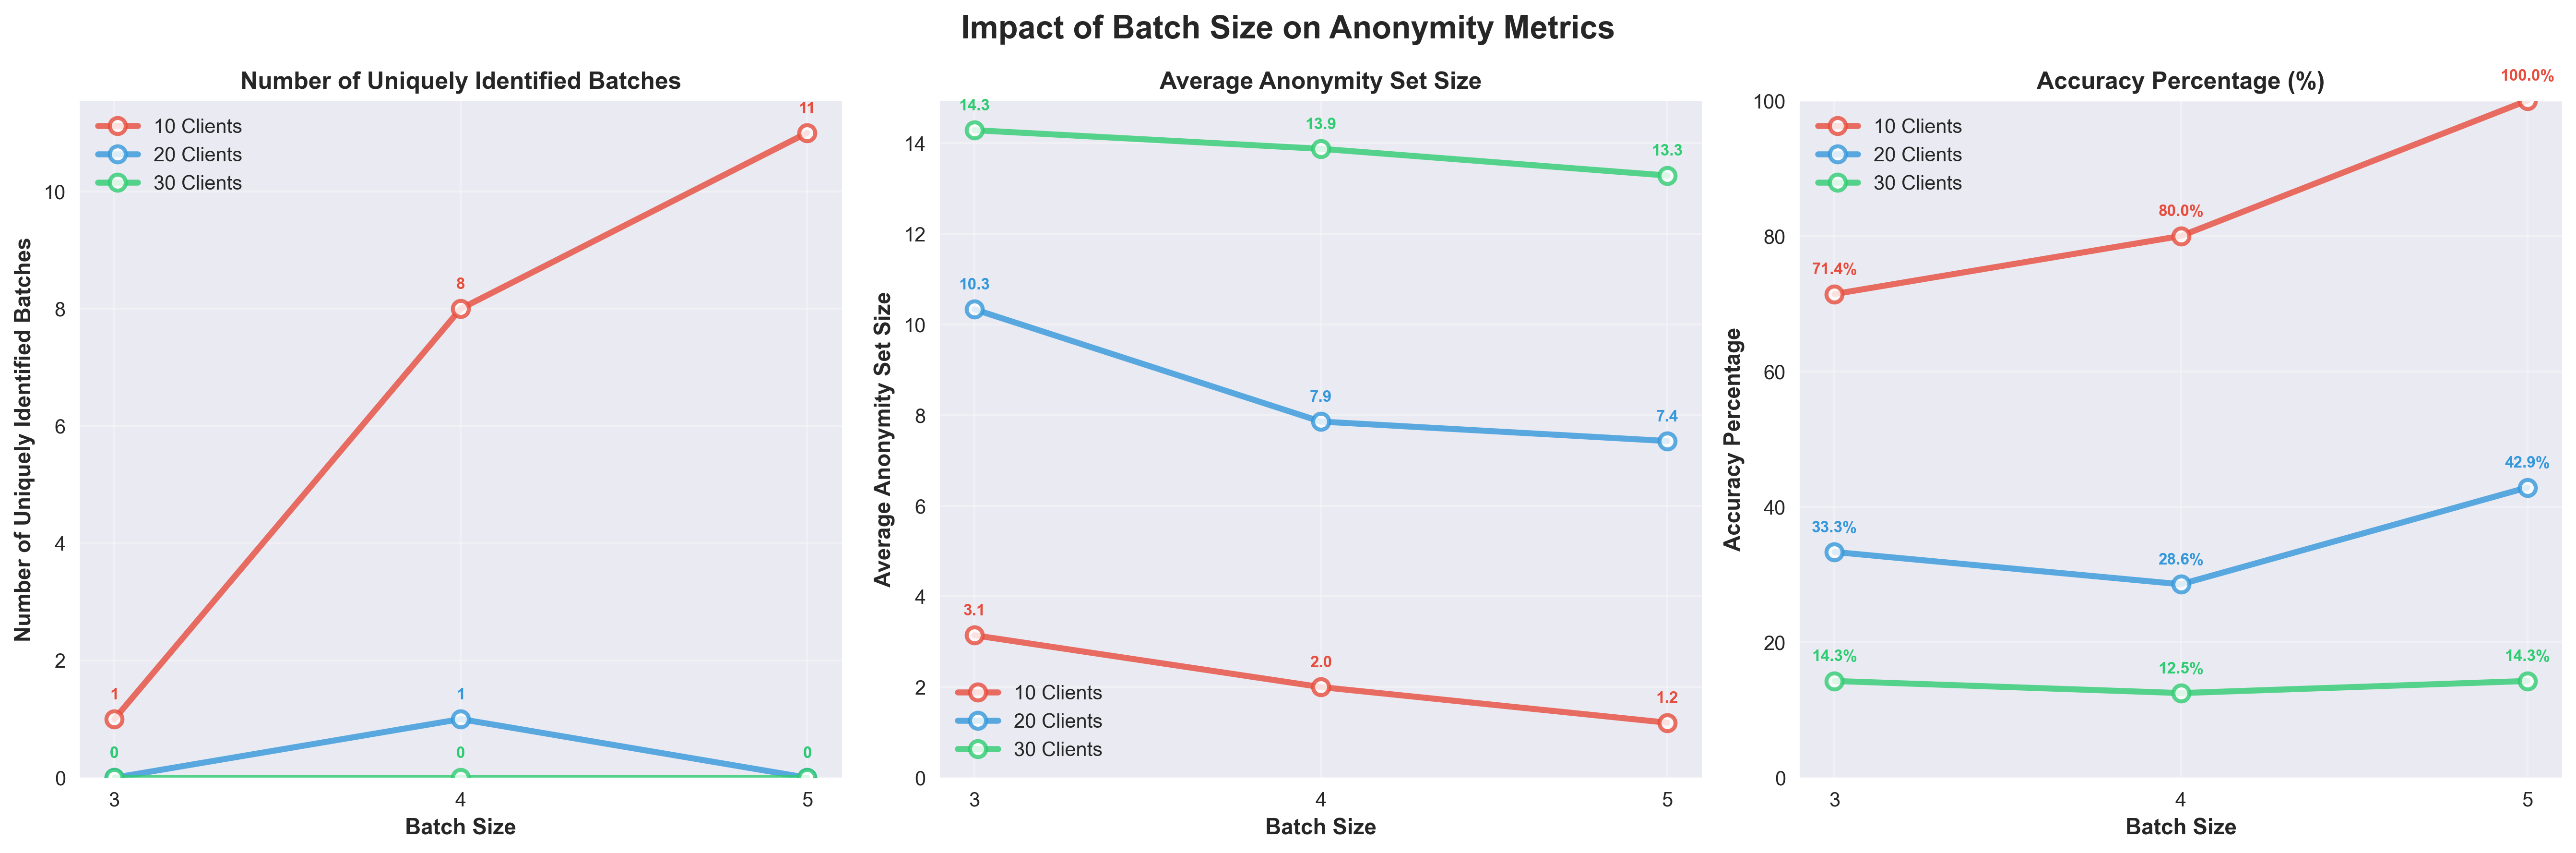
\includegraphics[width=0.8\textwidth]{diagrams/batch_size_analysis_combined.png}
\caption{Impact of batch size on various anonymity metrics across 
different numbers of clients (10, 20, and 30 clients). 
The plots show how batch size affects the number of uniquely 
identified batches, average anonymity set size, and accuracy percentage.}
\label{fig:batchsize_analysis}
\end{figure}

\subsection{Experimental Setup}

Due to the computational complexity of enumerating all valid batch 
permutations and the resulting scalability limitations, we 
conducted a limited set of fixed runs for each parameter 
configuration. The experimental design covers the following 
parameter space:

\begin{itemize}
\item \textbf{Number of clients:} 10, 20, and 30 clients
\item \textbf{Batch sizes:} 3, 4, and 5 messages per batch
\item \textbf{Mix node configuration:} Single Poisson mix node
\item \textbf{Simulation approach:} Fixed runs per configuration 
due to computational constraints
\end{itemize}

The evaluation metrics include the number of uniquely identified 
batches, average anonymity set size, and mapping accuracy percentage. 
These metrics provide insights into the anonymity guarantees offered 
by the mixnet under different parameters.

\subsection{Observations}

\subsubsection{Impact of Batch Size on Anonymity Metrics}

Figure~\ref{fig:batchsize_analysis} presents an analysis 
of how batch size affects anonymity across different 
client populations. 

For systems with 10 clients 
(red line), increasing batch size from 3 to 5 results in a 
degradation of anonymity: the number of uniquely 
identified batches increases from 1 to 11, the 
average anonymity set size decreases from 3.1 to 1.2, and the 
accuracy percentage rises from 71.4\% to 100\%, 
indicating that larger batches make it easier for 
adversaries to correlate incoming and outgoing traffic. 

In contrast, systems with 20 clients (blue line) show more 
complex behavior with some improvement in anonymity metrics 
at intermediate batch sizes, while systems with 30 clients 
(green line) maintain consistently strong anonymity across 
all batch sizes, with zero uniquely identified batches, 
stable anonymity set sizes around 13-14, and low accuracy 
percentages around 12-14\%. This suggests that the impact 
of batch size on anonymity is dependent on the number 
of participating clients, where smaller client populations 
become increasingly vulnerable to traffic analysis as batch 
sizes increase, while larger client populations provide 
sufficient mixing entropy to maintain privacy regardless 
of batch size.

\begin{figure}
\centering
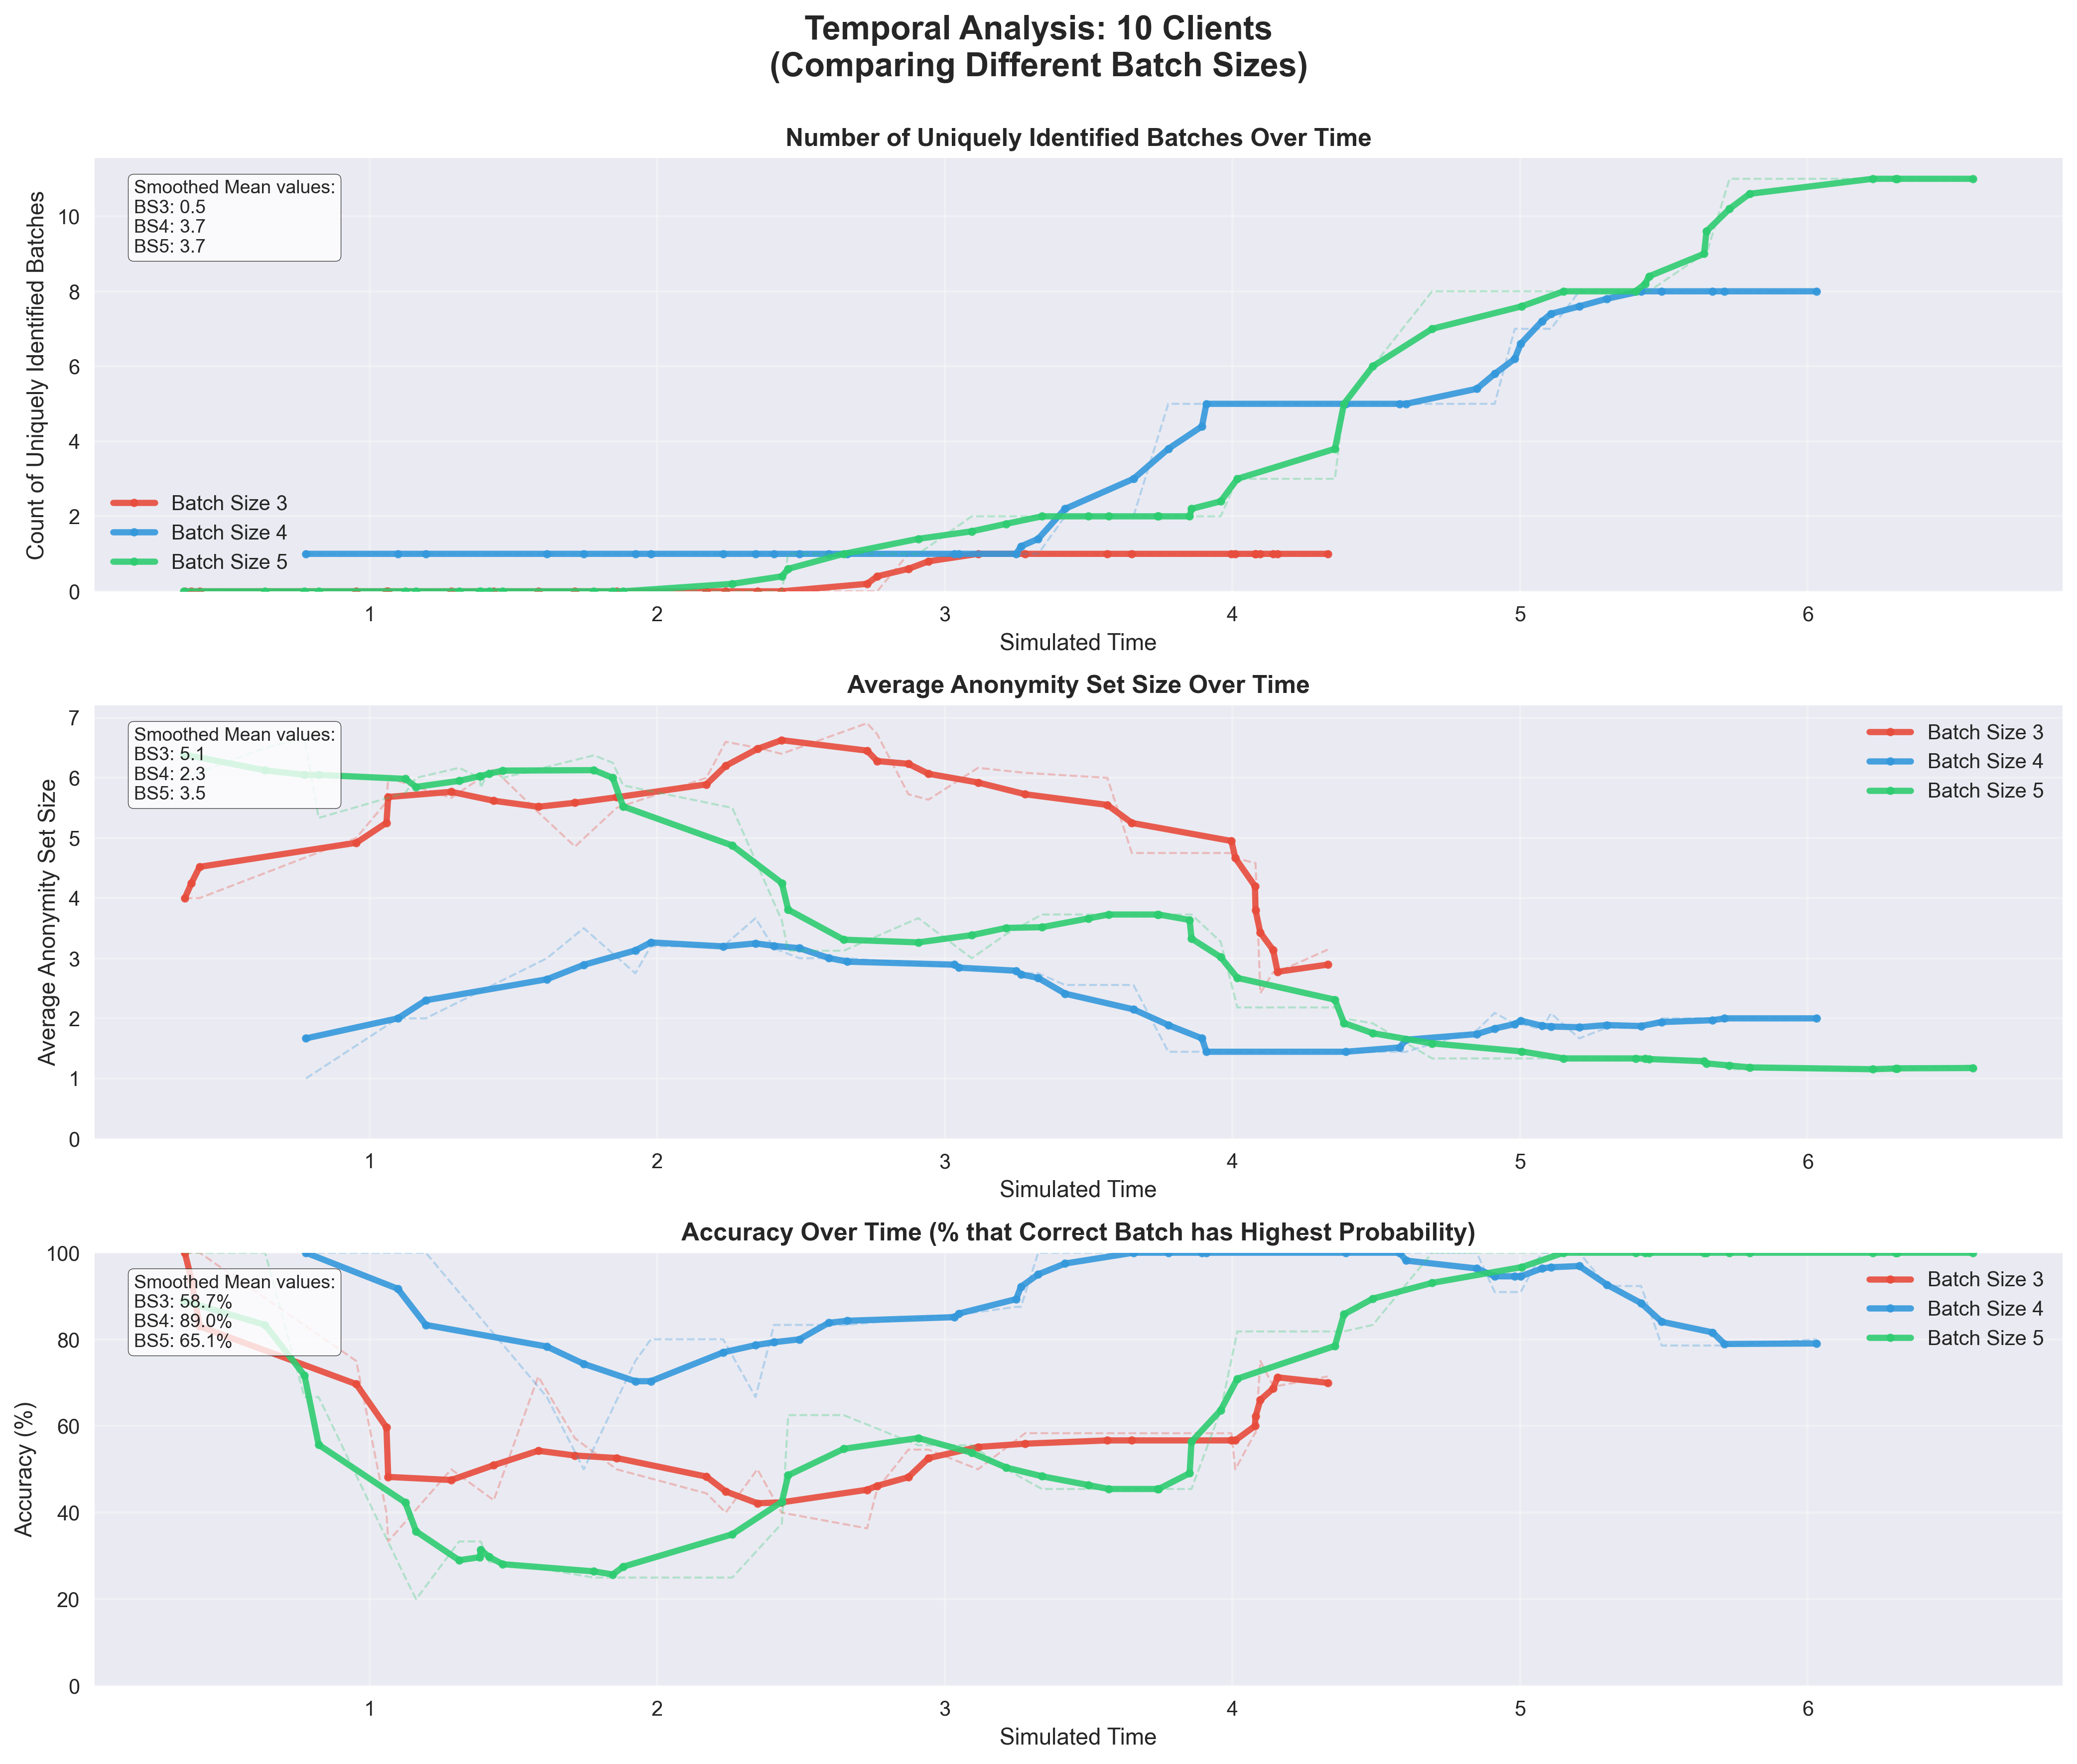
\includegraphics[width=0.8\textwidth]{diagrams/temporal_5_smoothed_10_clients.png}
\caption{Temporal analysis of anonymity metrics for 10 clients across different batch sizes (3, 4, and 5).}
\label{fig:temporal_analysis_10}
\end{figure}

\begin{figure}
\centering
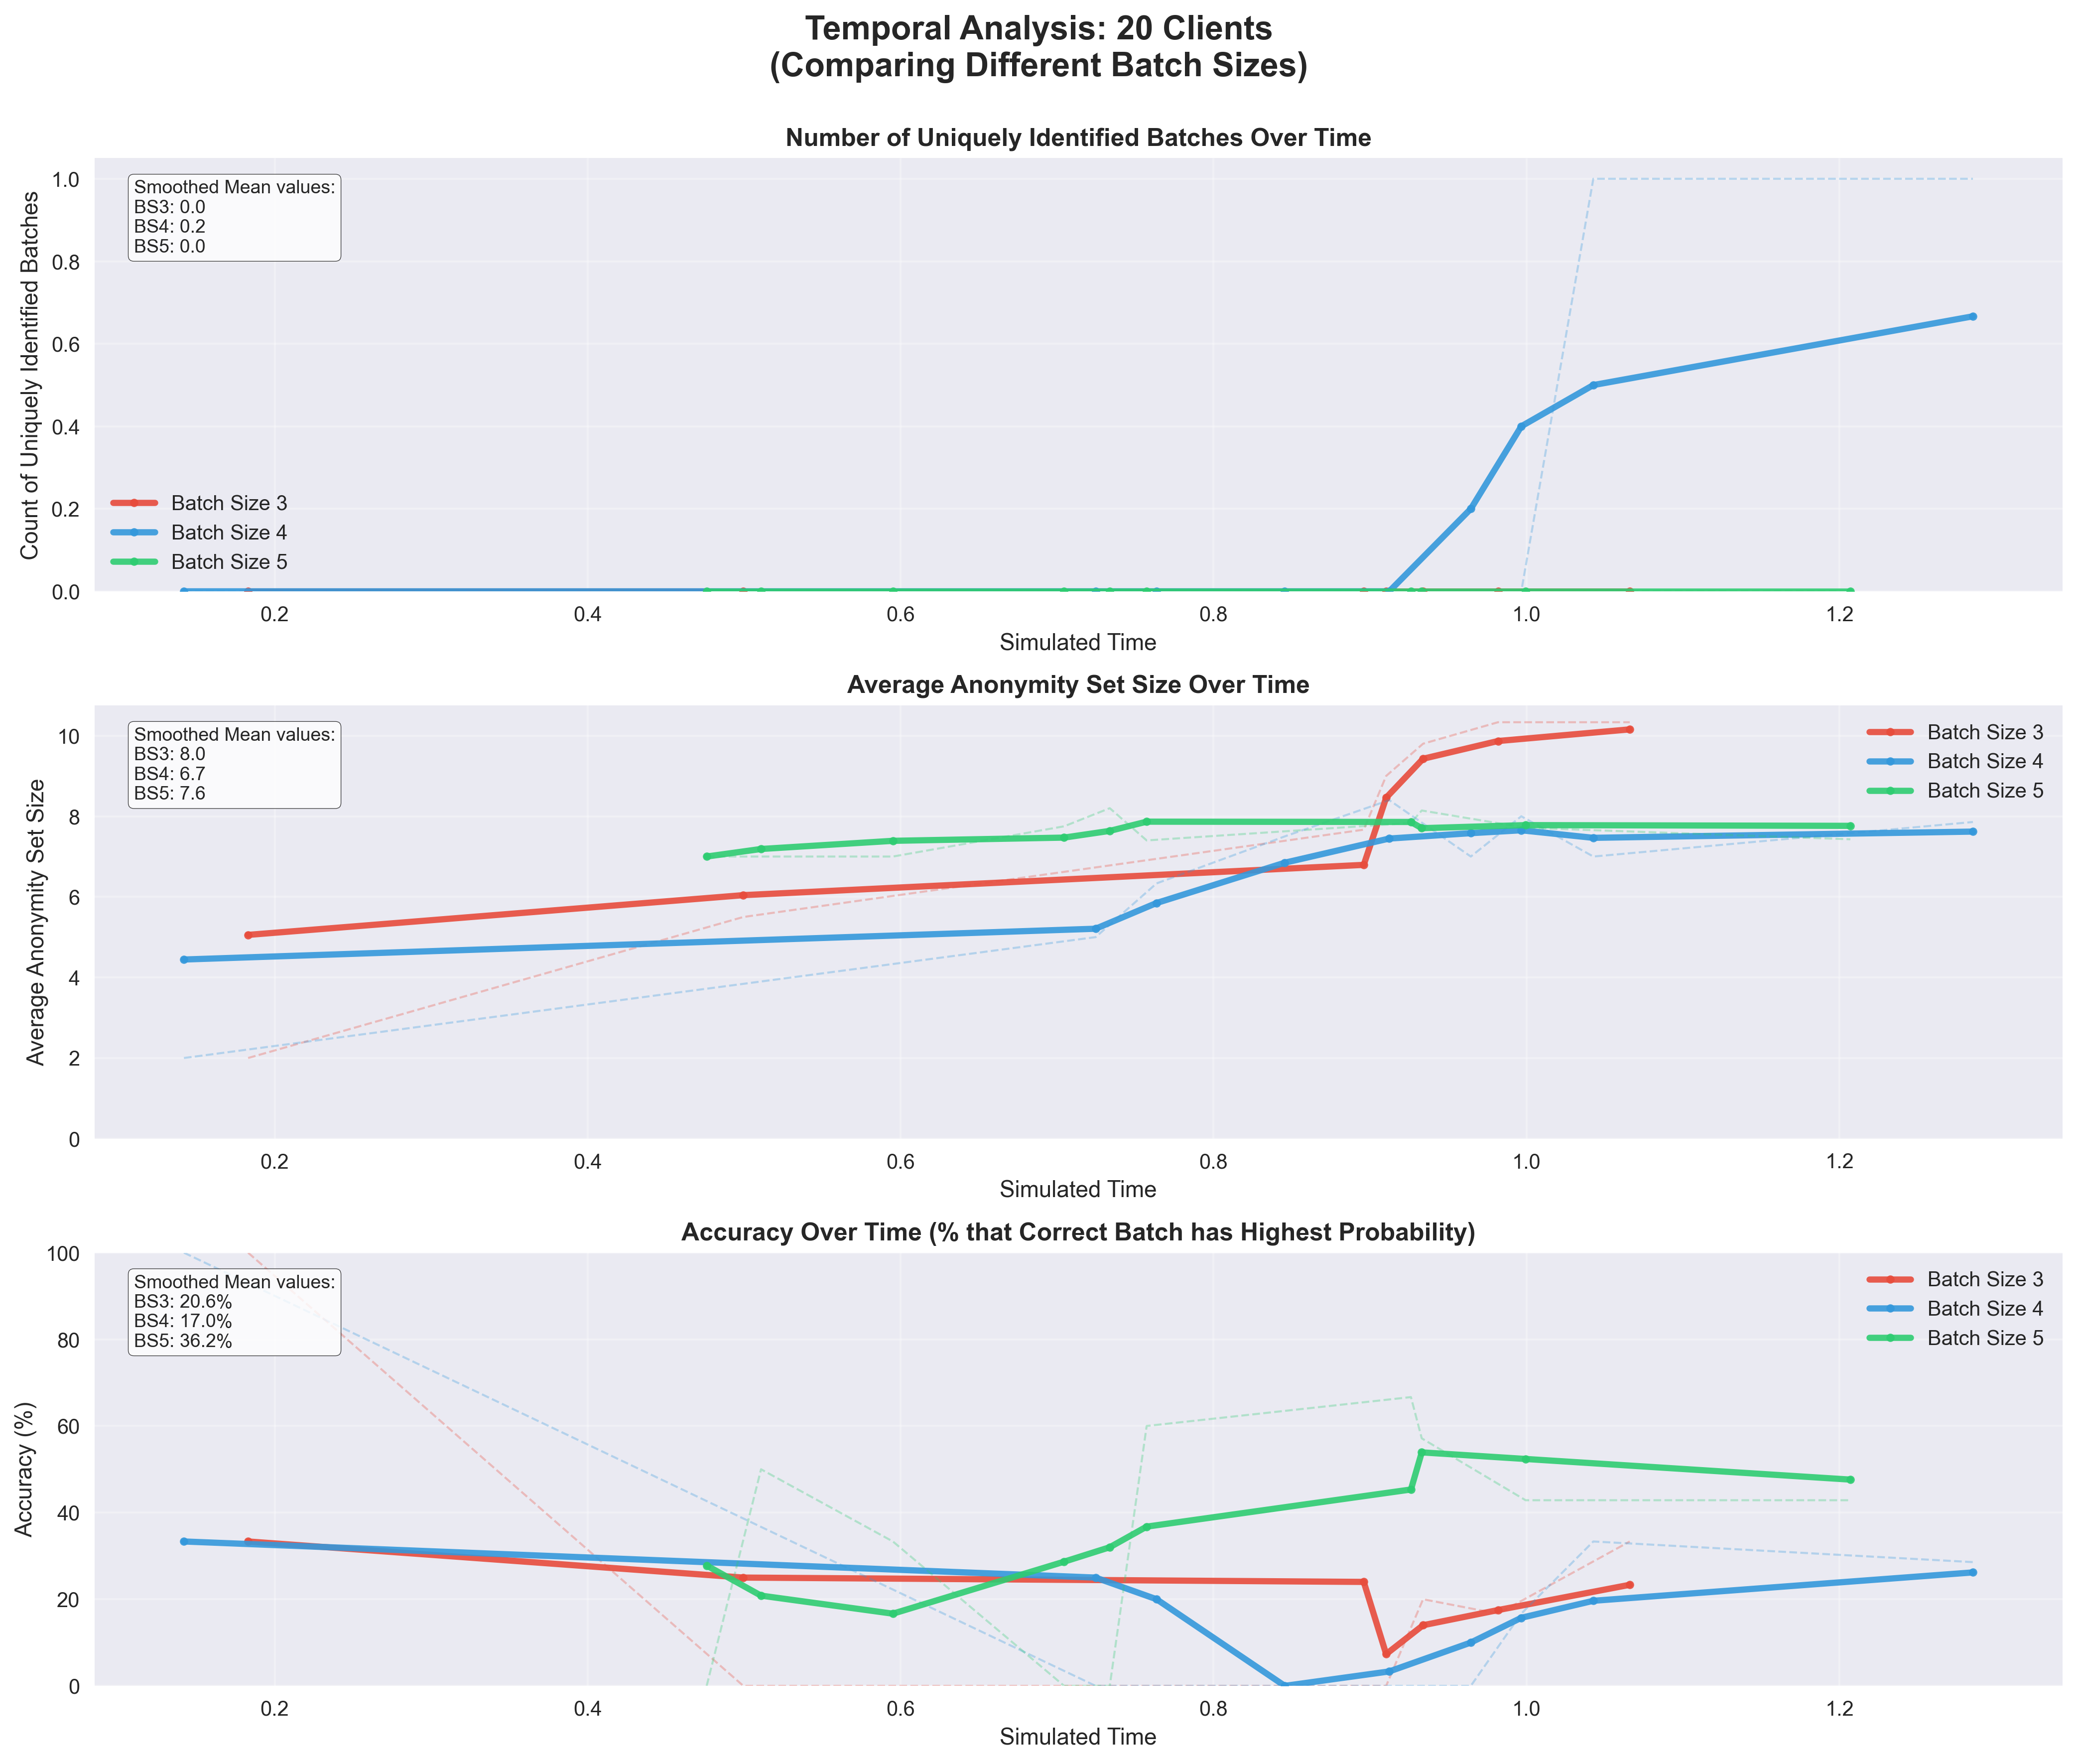
\includegraphics[width=\textwidth]{diagrams/temporal_5_smoothed_20_clients.png}
\caption{Temporal analysis of anonymity metrics for 20 clients across different batch sizes (3, 4, and 5).}
\label{fig:temporal_analysis_20}
\end{figure}

\begin{figure}
\centering
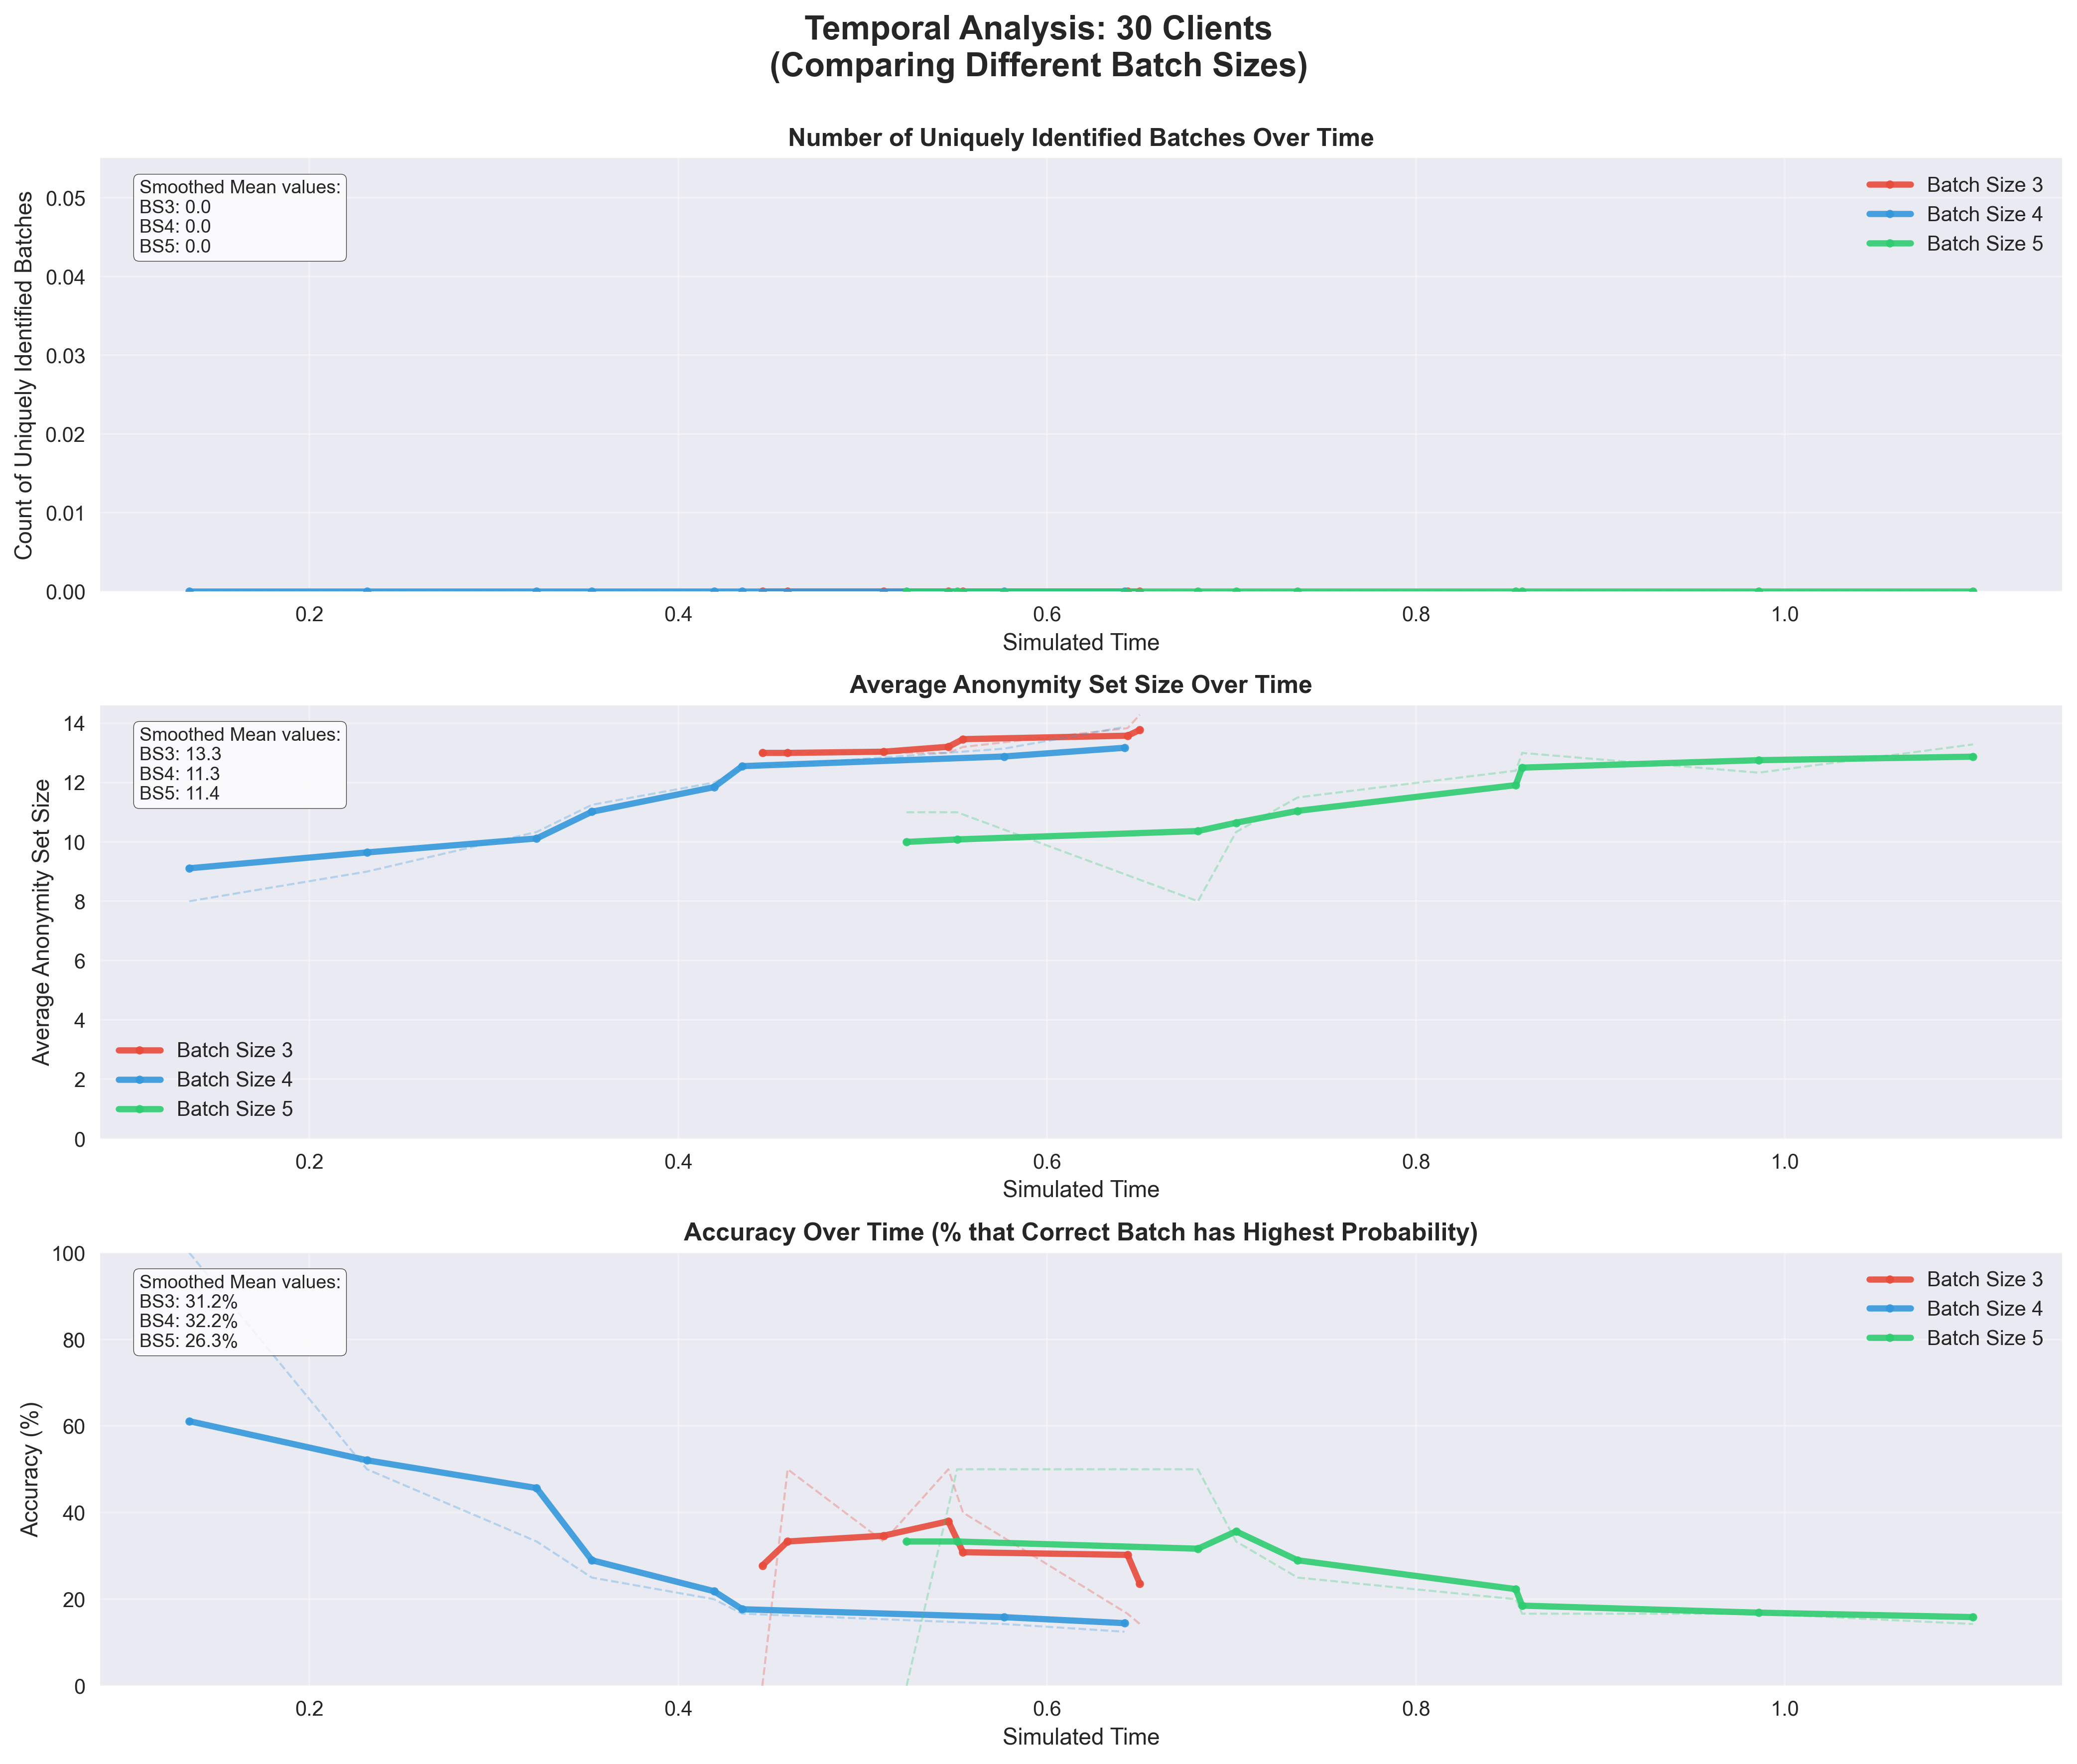
\includegraphics[width=\textwidth]{diagrams/temporal_5_smoothed_30_clients.png}
\caption{Temporal analysis of anonymity metrics for 30 clients across different batch sizes (3, 4, and 5).}
\label{fig:temporal_analysis_30}
\end{figure}

% \centering
% 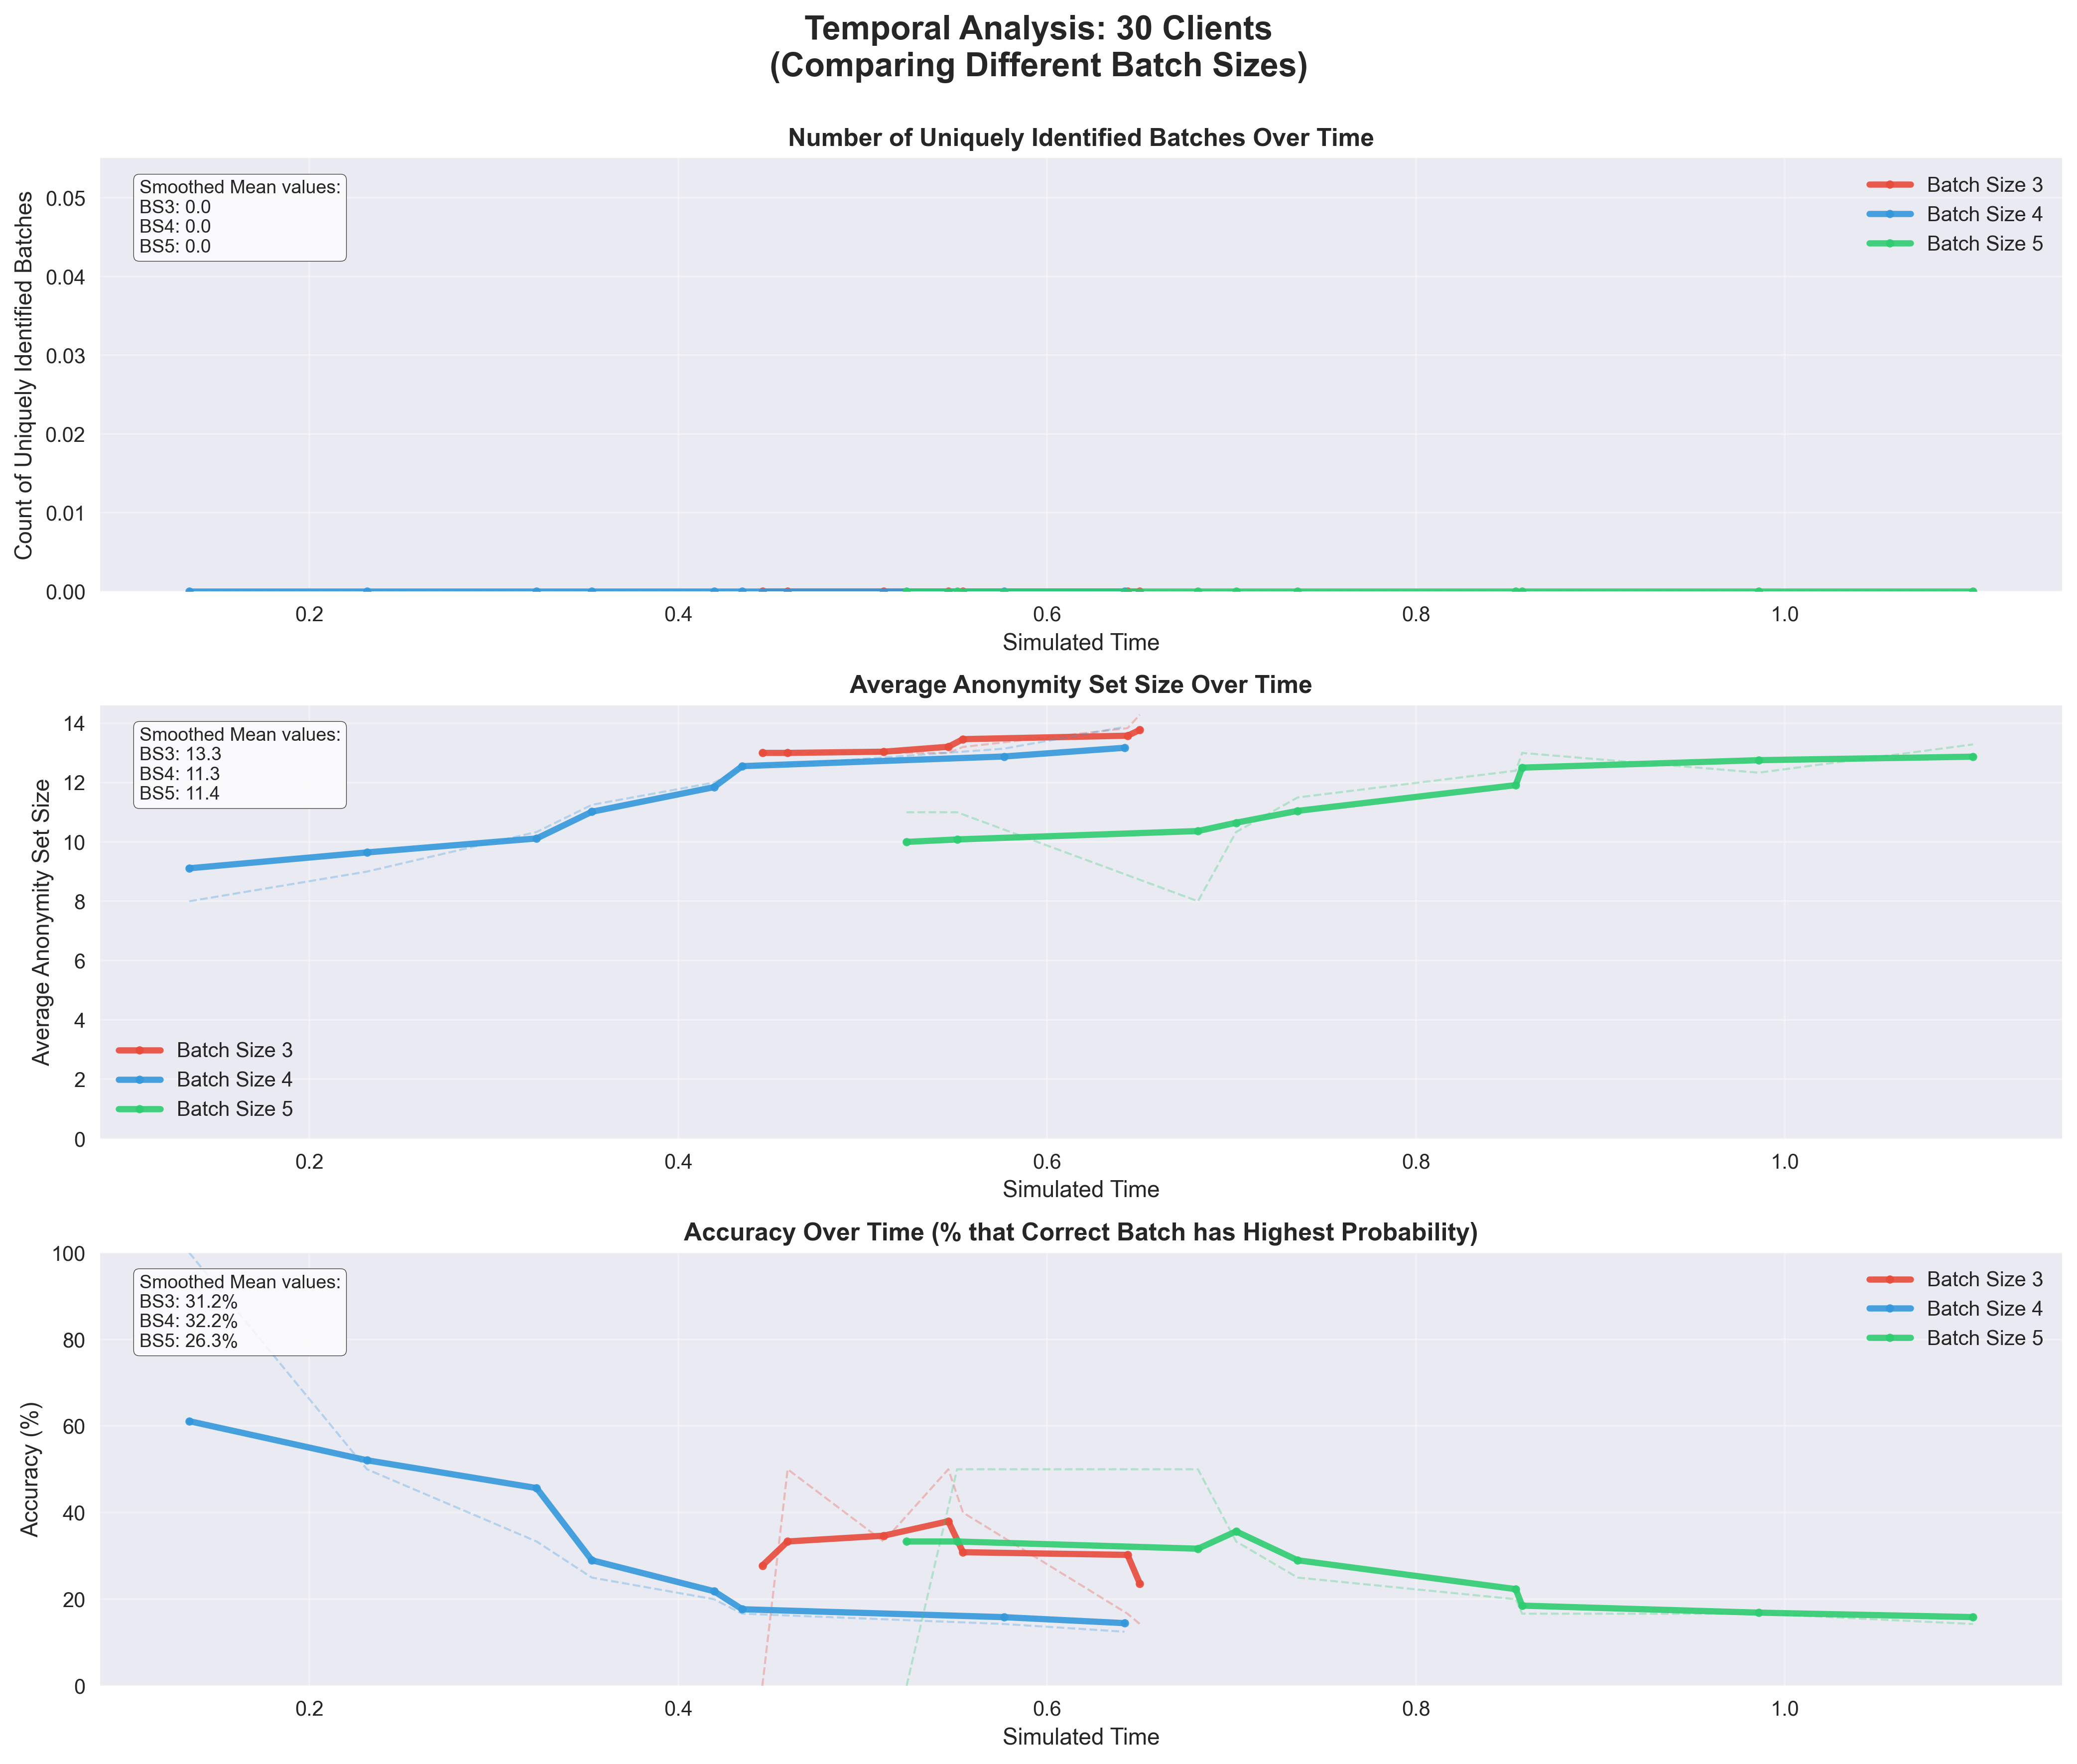
\includegraphics[width=\textwidth]{diagrams/temporal_5_smoothed_30_clients.png}
% \caption{Temporal analysis of anonymity metrics for 30 clients across different batch sizes (3, 4, and 5).}
% \label{fig:temporal_analysis_30}
% \end{figure*}

\subsubsection{Temporal Analysis}

The temporal analysis reveals how anonymity metrics evolve 
over time for different system configurations. 
Figures~\ref{fig:temporal_analysis_10}, \ref{fig:temporal_analysis_20}, 
and \ref{fig:temporal_analysis_30} show the temporal patterns 
for 10, 20, and 30 clients respectively, with smoothed curves 
for different batch sizes. 

The smoothing was applied to reduce noise and highlight 
underlying trends in the temporal data. A moving average 
filter with a window size of 5 data points was used 
to smooth the raw measurements. 

% This approach helps identify long-term 
% patterns while filtering out short-term fluctuations 
% that may be due to simulation randomness rather than 
% systematic behavior.

For 10 clients (Figure~\ref{fig:temporal_analysis_10}), 
the temporal patterns show significant variation in anonymity 
metrics over time, with different batch sizes exhibiting 
distinct trajectories. The smaller client population appears 
to create more volatile anonymity guarantees. The 20-client 
configuration (Figure~\ref{fig:temporal_analysis_20}) 
demonstrates more stable temporal patterns, with the anonymity 
metrics showing smoother evolution over time. This suggests 
that moderate client populations may provide a good balance 
between mixing effectiveness and system stability. With 30 clients 
(Figure~\ref{fig:temporal_analysis_30}), the temporal analysis 
reveals the most consistent anonymity patterns across different 
batch sizes, indicating that larger client populations contribute 
to more predictable privacy guarantees.

\subsubsection{Variation Between Runs}

Figure~\ref{fig:temporal_analysis_20_4_runs} shows multiple 
runs of the same parameter configuration (20 clients, batch size 4) 
to assess the variability and consistency of results across 
independent simulation runs.

\begin{figure}[!htb]
\centering
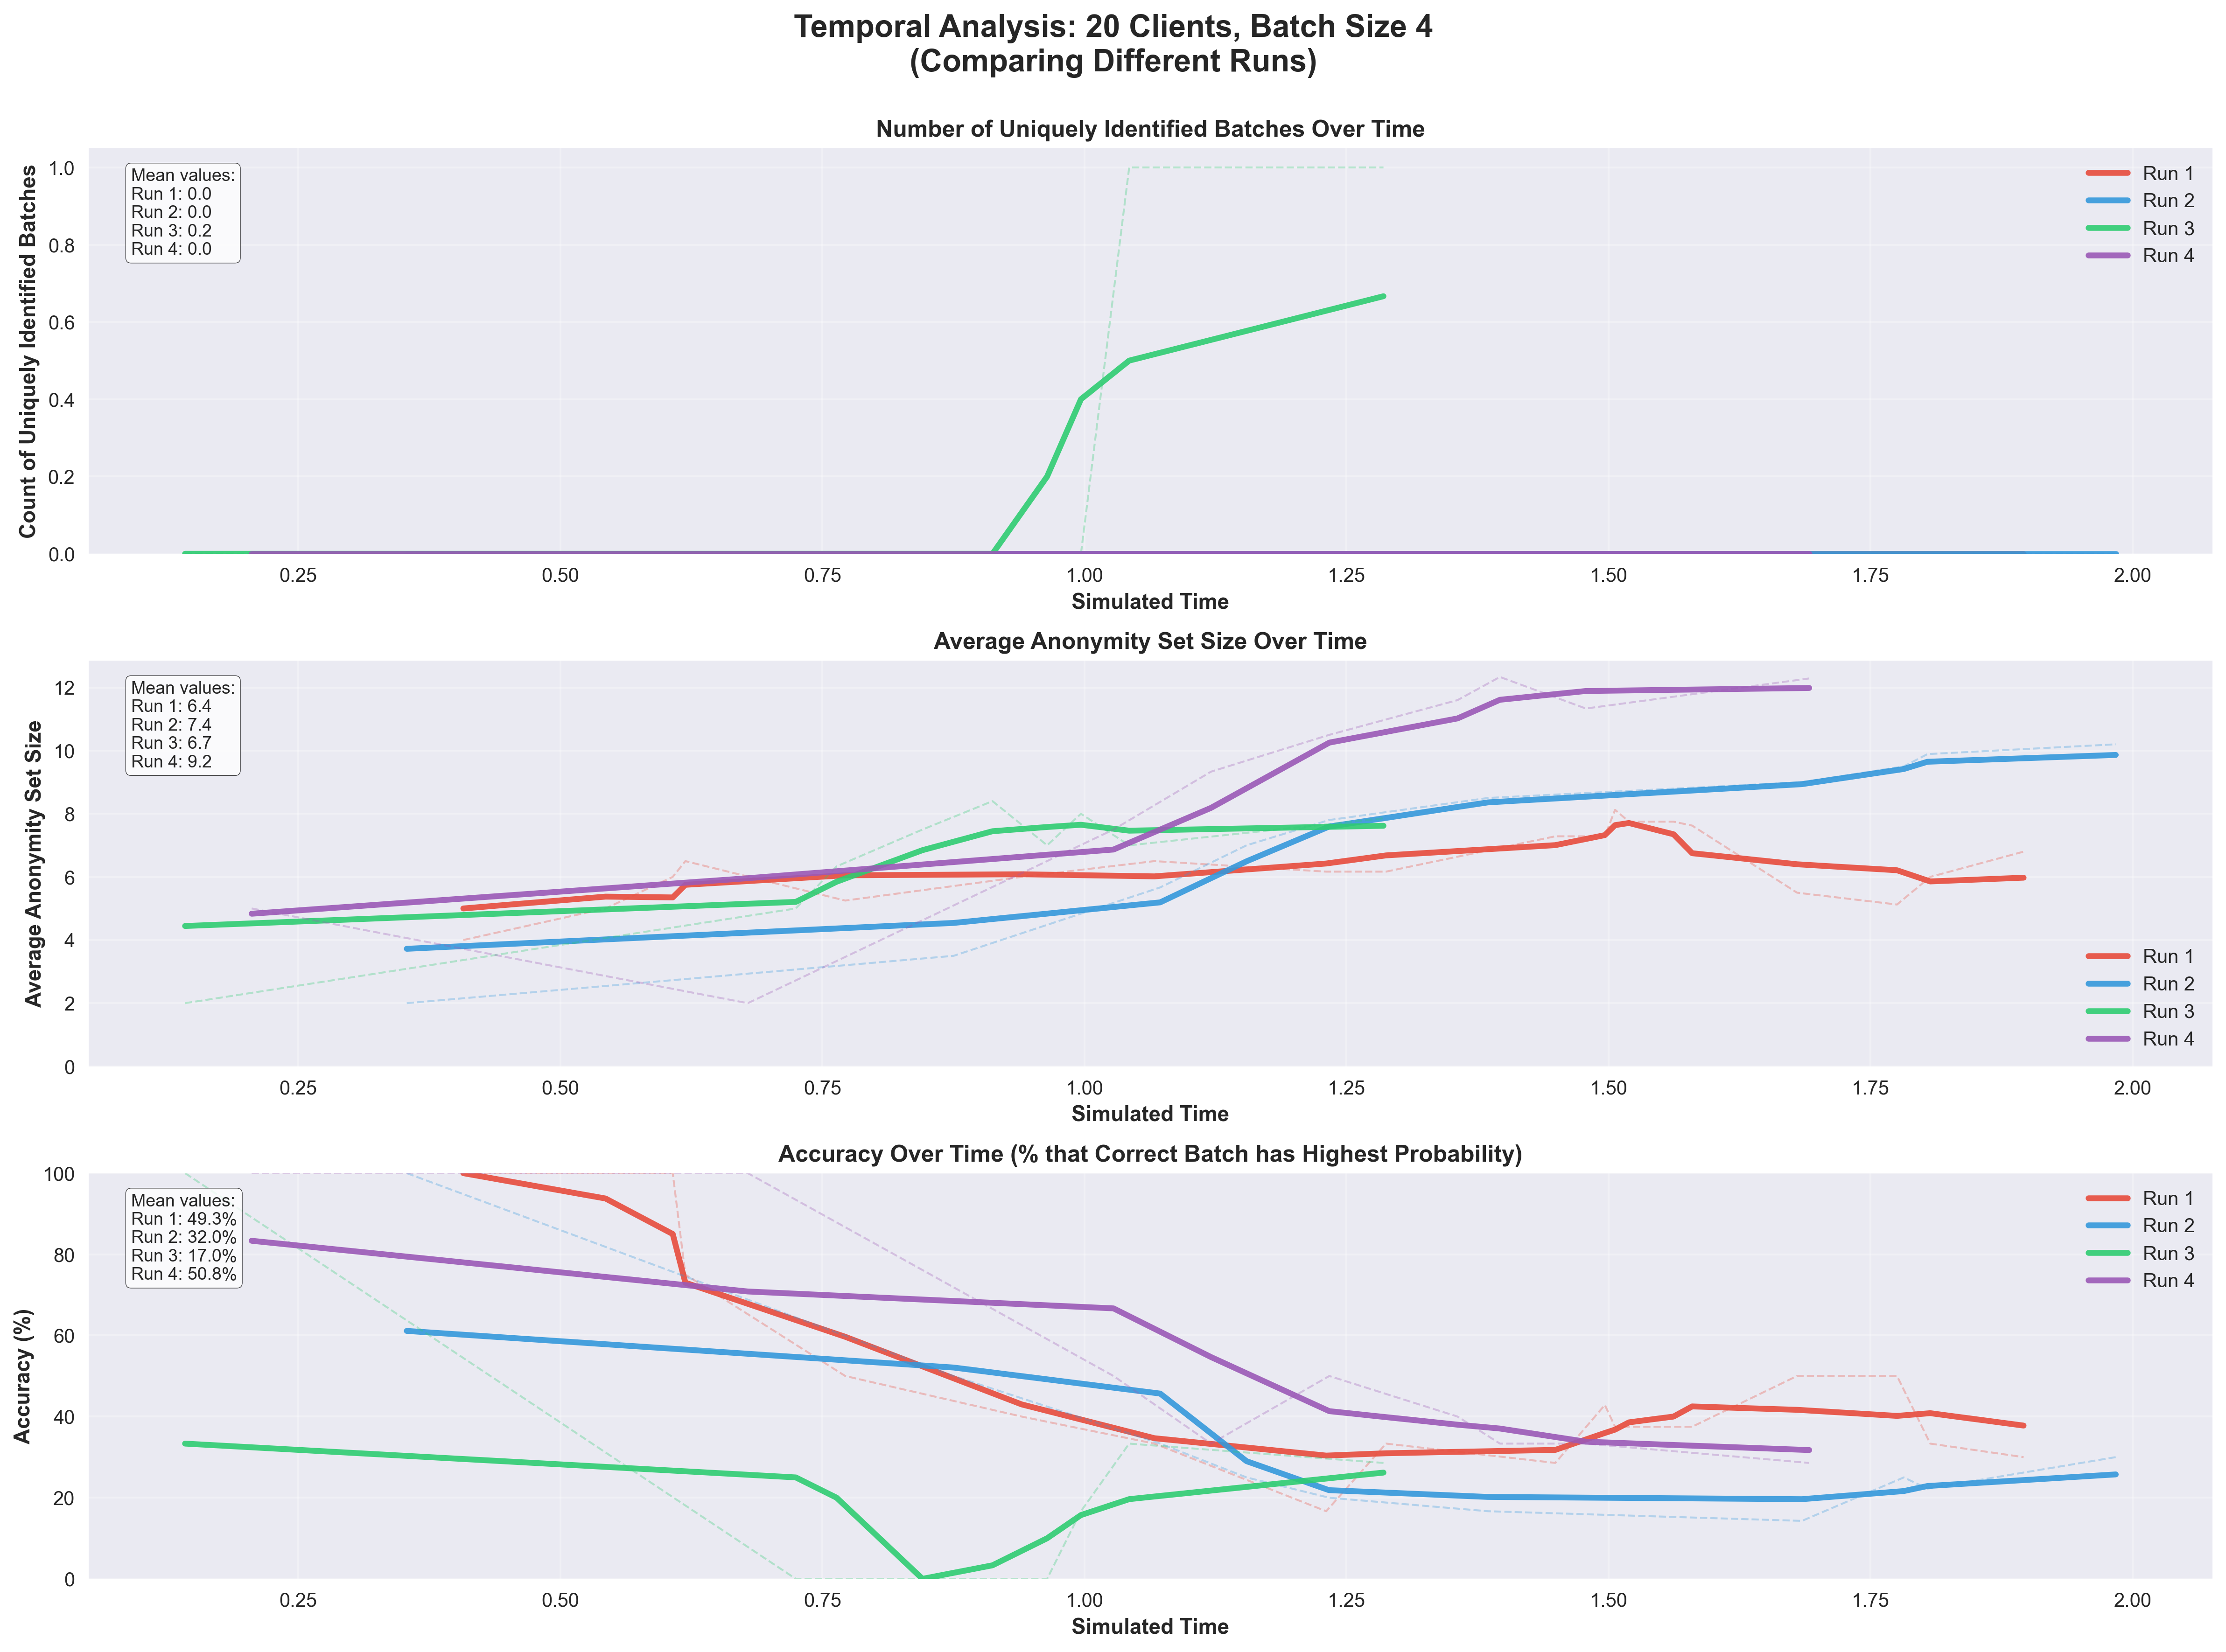
\includegraphics[width=\textwidth]{diagrams/temporal_20client_4batch_runs.png}
\caption{Temporal evolution of anonymity metrics across four independent simulation runs with identical parameters (20 clients, batch size 4).}
\label{fig:temporal_analysis_20_4_runs}
\end{figure}

The comparison reveals some variation between runs, highlighting 
the stochastic nature of the mixnet simulation and the importance 
of conducting multiple experiments for robust conclusions. The 
variation analysis across four independent runs reveals 
significant variability due to simulation randomness, with Run 3 
showing notably different behavior (uniquely identified batches 
climbing to 0.6 vs. near zero for others) and accuracy percentages 
varying dramatically from 20-100\% across runs. While anonymity 
set sizes show moderate 
consistency (6-12 range), the substantial differences 
in privacy outcomes demonstrate that identical system 
parameters can produce vastly different results depending 
on random simulation events. This illustrates the challenges in drawing 
definitive conclusions from limited experimental runs.


\subsection{Conclusion}
% \textbf{Conclusion:} 
It is important to note that due to computational limitations 
and the exponential complexity of the batch matching algorithm, 
our evaluation is based on a limited set of experimental runs. 
The patterns observed in this study should be interpreted with 
caution, as they represent only a small sample of the possible 
parameter space.

The computational complexity of enumerating all valid permutations 
scales poorly with both the number of clients and batch size, 
limiting our ability to conduct extensive statistical analysis. 
Additionally, the single-run approach for most configurations 
prevents us from establishing statistical significance or 
confidence intervals for our observations.

Future work should focus on developing more efficient algorithms 
that can handle larger parameter spaces and enable comprehensive 
statistical evaluation of anonymity guarantees under various 
operational conditions.

\end{document}